\begin{figure}[!h]
	\centering
	\subbottom[original image\label{fig:chbfrseg}]{
		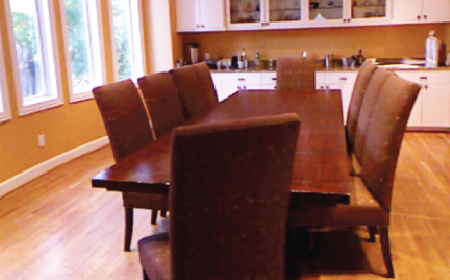
\includegraphics[width=\figfigfig\textwidth]{1-02-0.png}
	}
	\subbottom[semantic segmentation\label{fig:chsemseg}]{
		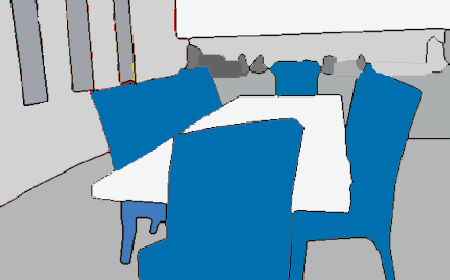
\includegraphics[width=\figfigfig\textwidth]{1-02-1.png}
	}
	\subbottom[instance segmentation\label{fig:chinsseg}]{
		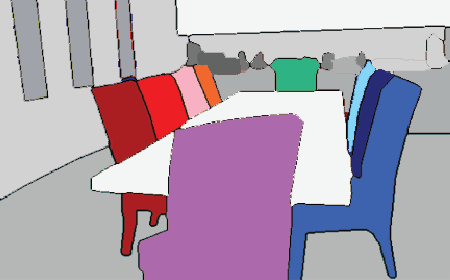
\includegraphics[width=\figfigfig\textwidth]{1-02-2.png}
	}
    \caption[Examples of semantic and instance segmentation]{Examples of semantic segmentation and instance segmentation. Image copyright owned by \cite{chaireccv}. The original image (a) shows a room with several chairs. (b) is the semantic segmentation result of (a), where blue color denotes the chairs, and other colors such as white and gray denote irrelevant background. (c) is instance segmentation result of (a), where all chairs have the same label, but different colors which are used to indicate different instances.}
	\label{fig:chseg}
\end{figure}